\chapter{Resultados e Discussão}\label{cap:resultados}

\section{Sequenciamento e controle de qualidade das leituras}
Após o sequenciamento das amostras, foram obtidas 7.8 milhões de leituras de tamanho médio de 
223 pares de base para a amostra ACT016 e 7.4 milhões de leituras com tamanho médio de 222 pares de base
para a amostra ACT094. Após a filtrar as leituras utilizando a ferramenta Trimmomatic, retivemos
6.2 milhões de leituras com tamanho médio 113 pares de base \(perda 21,5\%\) para ACT016 e 6.1 milhões
de leituras com tamanho médio 145 pares de base\(perda de 18,5\%\).

Baseando-se num tamanho de genoma variável de 3 a 10 milhões de bases para \textit{Rhodococcus}, podemos
determinar a cobertura real estimada pela fórmula $C= (L\cdot N)/G $ sendo $C$ a cobertura, $L$ o comprimento
médio das reads e $G$ o tamanho do genoma. A partir disso, obtivemos que a cobertura para a amostra ACT016 Após
filtrar as leituras está entre $70$ e $233,53$ vezes. 
Para a amostra ACT094, consideramos o tamanho do genoma de referência de \textit{Brevibacillus Brevis}$($NZ\_LR134338$)$ 
de 6.2 milhões de bases e estimamos a cobertura em aproximadamente $142,66$ vezes.

As qualidades médias das sequências pode ser observada a partir dos gráficos a seguir gerados pela ferramenta FASTQC:

\begin{figure}[H]
	\caption{Gráficos representando a qualidade média das leituras da amostra ACT016 na escala PHRED}
	\centering
	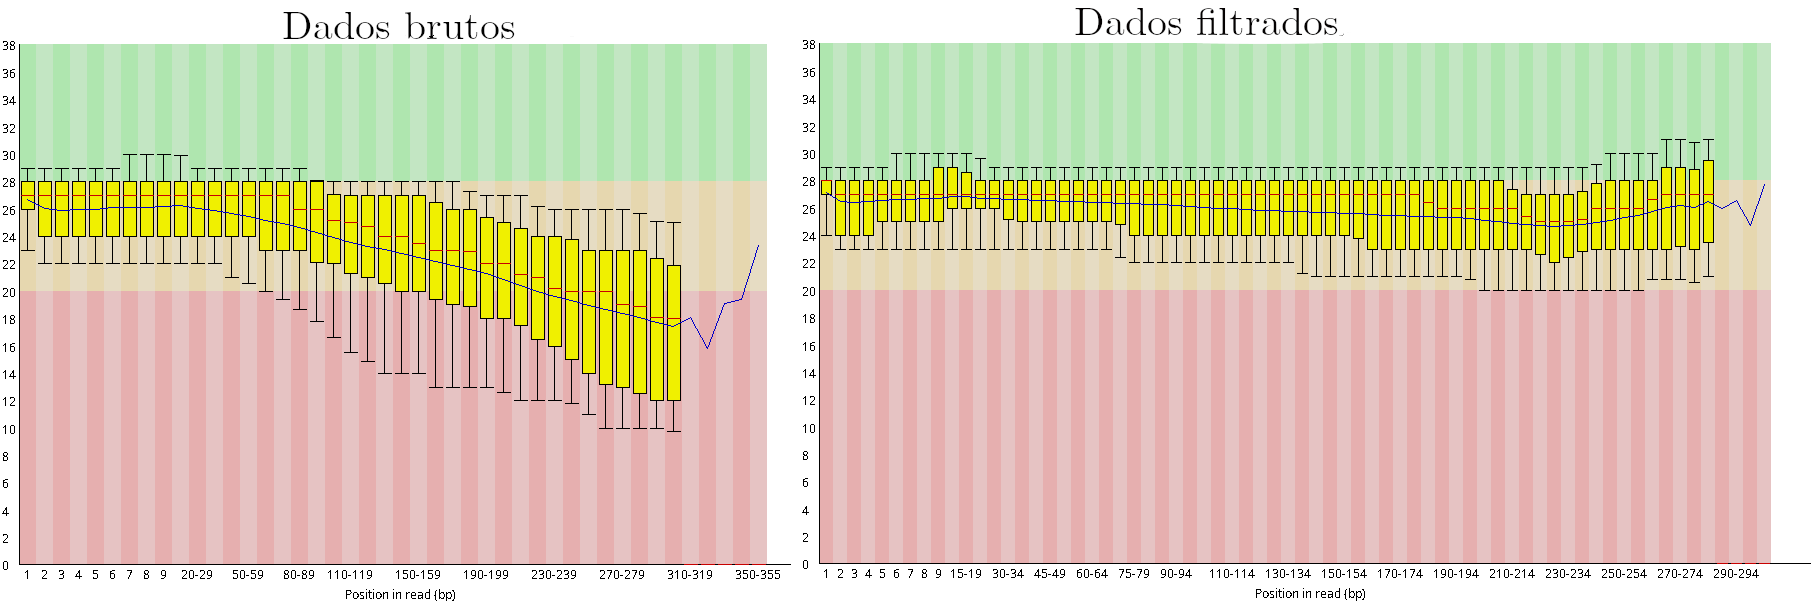
\includegraphics[width=0.8\linewidth]{imagens/read\_qc/002merged.png} \\
	\centering
    \begin{small}\textbf{Fonte: O Autor (2022)}\end{small}
\end{figure}
\vspace{\floatsep}
\begin{figure}[H]
	\caption{Gráficos representando a qualidade média das leituras da amostra ACT094 na escala PHRED}
	\centering
	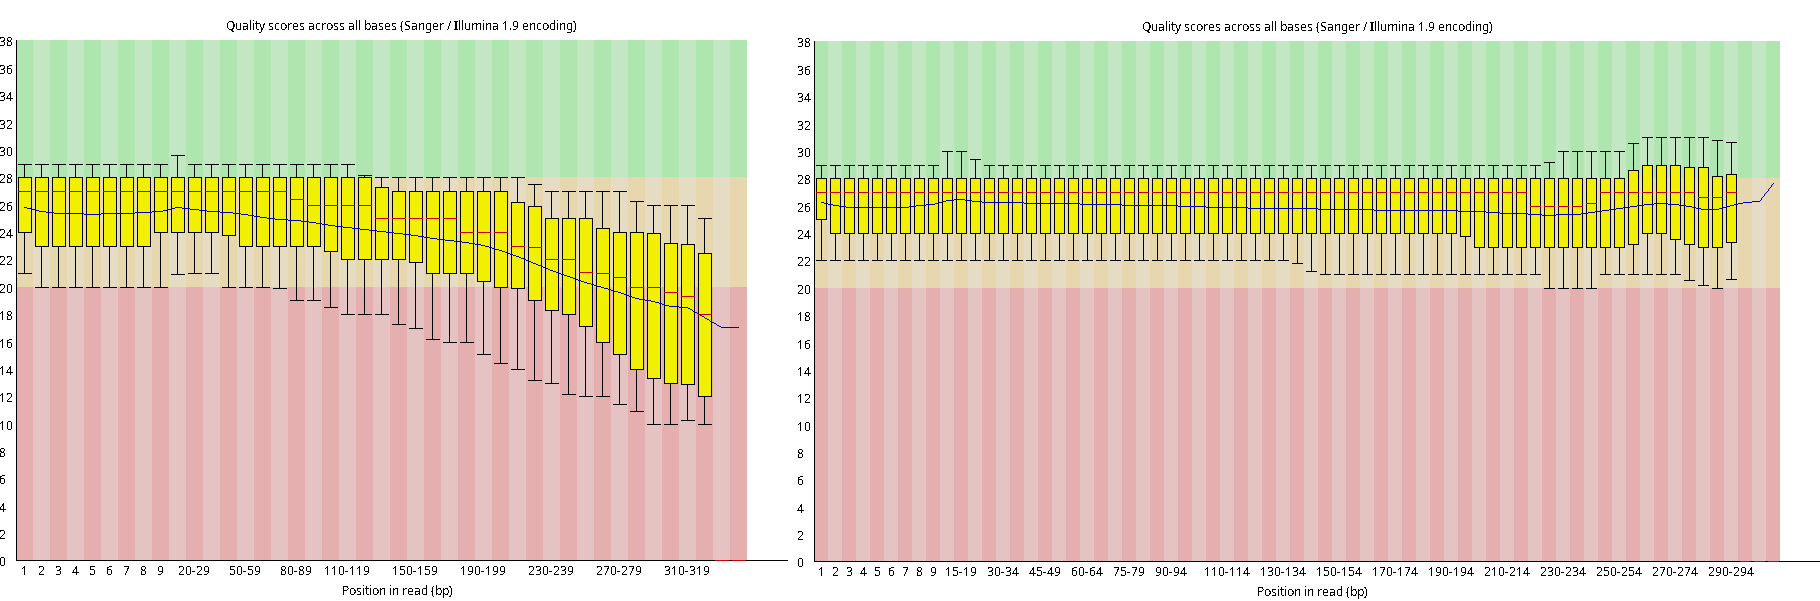
\includegraphics[width=0.8\linewidth]{imagens/read\_qc/004merged.png} \\
	\centering
    \begin{small}\textbf{Fonte: O Autor (2022)}\end{small}
\end{figure}
\vspace{\floatsep}

A partir desses gráficos podemos observar a perda de qualidade no final das leituras, um tipo de limitação
técnica comum ao utilizar sequenciadores da plataforma \textit{Illumina}, porém o término em baixa qualidade
pode ser removido após a filtração, tendo uma qualidade média ao longo da sequência próximo de PHRED 26 e
removendo sequências abaixo de PHRED 20 $($ que representa probabilidade de erro maior que 1 em 100$)$.


\section{Montagem das \textit{contigs}}

\begin{figure}[H]
	\caption{Report do software QUAST para as montagens da amostra 016}
	\label{fig:quast_16}
	\centering
		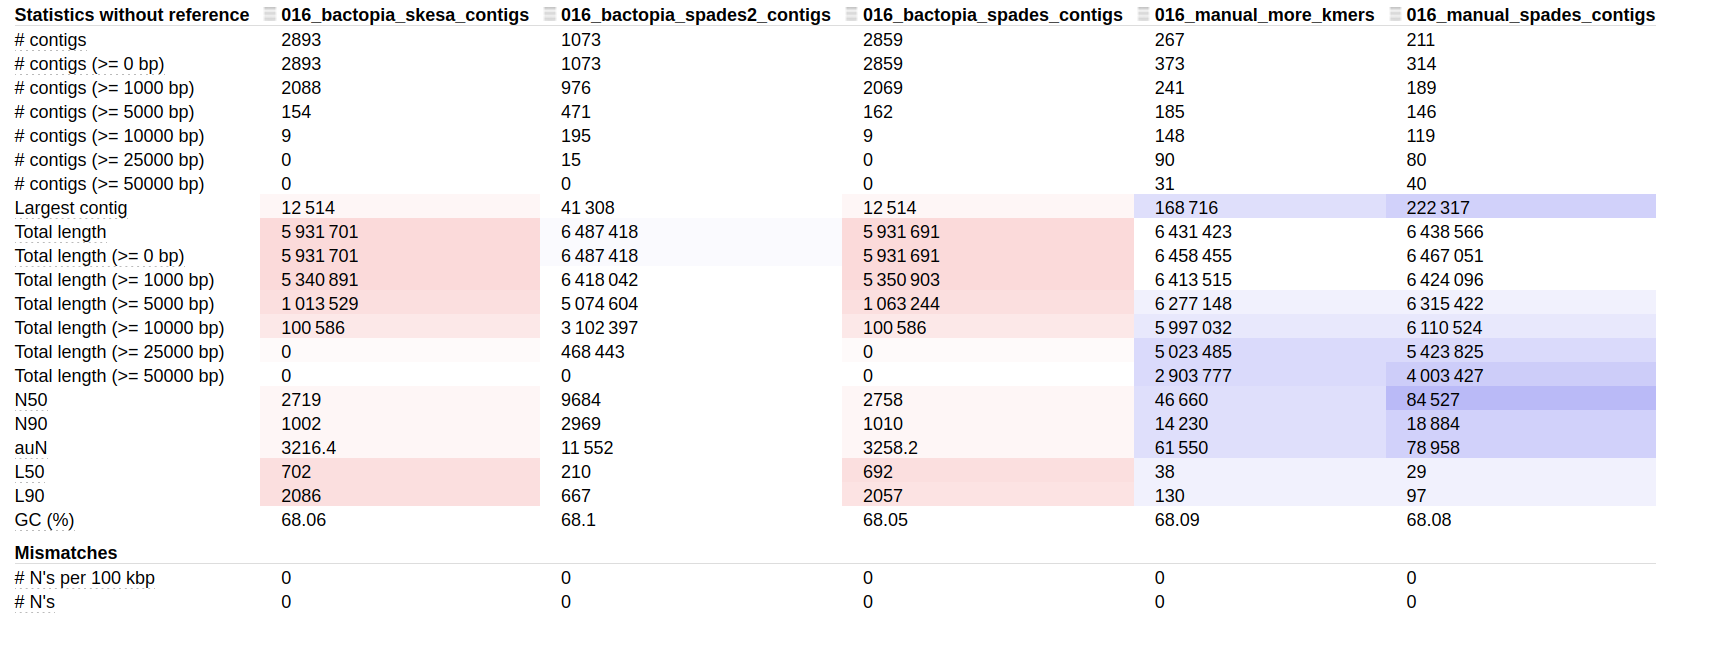
\includegraphics[width=0.8\linewidth]{imagens/assembly\_qc/016assembly.png} \\
	\centering
    \begin{small}\textbf{Fonte: O Autor (2022)}\end{small}
\end{figure}
\vspace{\floatsep}

A melhor montagem para a amostra ACT016 é a montagem \textit{manual\_spades} que foi feita utilizando
o montador spades junto com a correção do software shovill. Essa montagem foi escolhida por ter o maior
valor de L50 $($menor quantidade de contigs para atingir 50 \% do número de pares de base$)$ e maior 
\textit{contig} em tamanho absoluto $($222 mil pares de base$)$. O conteúdo GC de 60 \% dessa montagem está de acordo
com o descrito por \citeonline{yadav2018} para Actinomicetos.


\begin{figure}[H]
	\caption{Report do software QUAST para as montagens da amostra 094}
	\label{fig:quast_16}
	\centering
		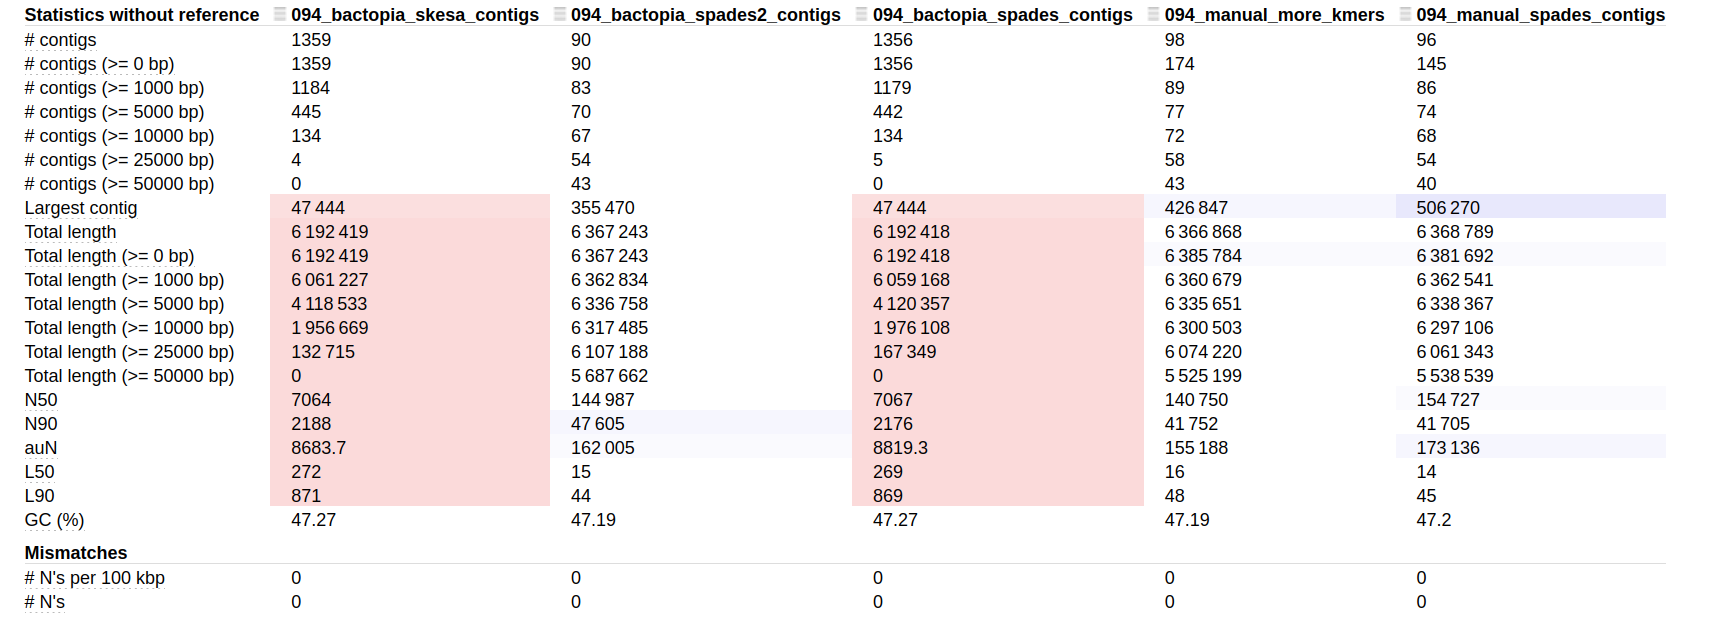
\includegraphics[width=0.8\linewidth]{imagens/assembly\_qc/094assembly.png} \\
	\centering
    \begin{small}\textbf{Fonte: O Autor (2022)}\end{small}
\end{figure}
\vspace{\floatsep}

De maneira similar, a melhor montagem para a amostra 094 também é a montagem \textit{manual\_spades}.
possuindo um valor similar a montagem \textit{more\_kmers} porém se diferenciando por possuir a maior \textit{contig}
com aproximadamente 80 mil pares de base a mais, um fator muito relevante para a posterior montagem do genoma completo.
O conteúdo GC também está de acordo com valores comumente encontrados em \textit{Brevibacillus brevis} \cite{nakamura1991bacillus}.

\section{Predição de espécies e montagem de genoma}

Os melhores conjuntos de \textit{contigs} montadas foram submetidas ao software KRAKEN2 para predição de espécie,
para a amostra 016 a espécie predita foram \textit{Rhodococcus} com $71,66$ \% de \textit{contigs} identificadas, mas importunamente
$18,45$ \% das \textit{contigs} não foram identificadas, determinando que a amostra 016 foi predita como \textit{Rhodococcus}
não identificado. A partir desse resultado o genoma de referência sugerido para a montagem foi o de código
de acesso NZ\_CP054690 da cepa \textit{Rhodococcus sp. W8901}. 

Para a amostra 094, $85.52$ \% das \textit{contigs} foram preditas como \textit{Brevibacillus brevis}
concordando com os resultados previamente obtidos a partir de sequenciamento de sanger. O genoma NZ\_CP030117
da cepa \textit{DZQ7} referência para montagem de genomas dessa espécie.

As montagens utilizando genomas de referência escolhidos, foram avaliadas quanto a presença de genes 
ortólogos. Na amostra 016 foram encontrados 120 BUSCOs completos e únicos, 2 genes completos e duplicados e 2 genes fragmentados,
 o valor de genes completos únicos de 98\% foi considerada satisfatória para a montagem e de pureza suficiente para
a anotação do genoma. Já na amostra 094, 121 BUSCOs completos e únicos foram encontrados, 1 gene completo e duplicado, 1 busco fragmentado
e 1 busco faltando, com o percentual de $98,4$ \% também foi considerada suficiente para prosseguimento da anotação.

o software PROKKA foi capaz de predizer 5738 CDSs para a amostra 016 e 6082 CDS para a amostra 094, contendo genes
de diversas funções celulares. 

\section{Predição de \textit{BGCs} e resistência a antimicrobianos}

Para a amostra 016, o software Antishmash foi capaz de identificar 16 cluster biosintéticos completos, porém
apenas um cluster foi predito com 75\% de similaridade para produção de ectoína, um produto biosintético
conhecido e produzido por uma ampla gama de bactérias gram positivas e negativas \cite{toveken2011specialized}.
Além disso, através da ferramenta armfinder foi observada a presença de genes codificando uma beta-lactamase de classe A e uma proteína de
proteção ribossomal ABC-F. A presença desses genes, pode indicar a resistência desse microorganismo a antibióticos beta-lactâmicos
e a macrolídeos.  

Já a amostra 094, teve 15 cluster biosintéticos preditos, dentro os quais 4 tiveram sua função identificada
por similaridade sendo produtores das seguintes substâncias e identidades percentuais: petrobactina$($83\%$)$, 
tyrocidina$($81\%$)$, gramicidina$($91\%$)$ e macrobrevina ($($100\%$)$). 


 \begin{figure}[H]
	\caption{\textit{Cluster biosintético} para produção de petrobactina na amostra 094}
	\label{fig:quast_16}
	\centering
		\includegraphics[width=0.8\linewidth]{imagens/antismash/094regiao1.svg} \\
	\centering
    \begin{small}\textbf{Fonte: O Autor (2022)}\end{small}
\end{figure}
\vspace{\floatsep}

A petrobactina é um sideróforo com protoreatividade capaz de reduzir ferro $III$ em 
ferro $II$\cite{barbeau2002petrobactin}. Interessantemente o cluster presente na amostra 94
capaz de produzir petrobactina, contém uma proteína de resistência tipo A a vancomicina e teicoplanina.

\begin{figure}[H]
	\caption{\textit{Cluster biosintético} para produção de tirocidina na amostra 094}
	\label{fig:quast_16}
	\centering
		\includegraphics[width=0.8\linewidth]{imagens/antismash/094regiao2.svg} \\
	\centering
    \begin{small}\textbf{Fonte: O Autor (2022)}\end{small}
\end{figure}
\vspace{\floatsep}

\begin{figure}[H]
	\caption{\textit{Cluster biosintético} para produção de gramicidina na amostra 094}
	\label{fig:quast_16}
	\centering
		\includegraphics[width=0.8\linewidth]{imagens/antismash/094regiao3.svg} \\
	\centering
    \begin{small}\textbf{Fonte: O Autor (2022)}\end{small}
\end{figure}
\vspace{\floatsep}

A gramicidina e tirocidina são peptídeos lineares de síntese não ribossomal, com mecanismo de ação
através do dano na membrana celular de outros organismos, a tirocidina é relatada como um candidato importante
a antibiótico de nova geração por não ter induzido resistência nas células afetadas\cite{yang2018antimicrobial}.
A presença de clusters capazes de produzir não apenas um mas dois tipos diferentes de peptídeos com
atividade antimicrobiana sugere atividade antimicrobiana no isolado 094, o que precisa ser elucidado através
de testes \textit{in vitro} em condições que promovam a expressão desses compostos para posterior purificação e
descrição de suas estruturas através da técnica de espectometria de massa.

\begin{figure}[H]
	\caption{\textit{Cluster biosintético} para produção de macrobrevina na amostra 094}
	\label{fig:quast_16}
	\centering
		\includegraphics[width=0.8\linewidth]{imagens/antismash/094regiao4.svg} \\
	\centering
    \begin{small}\textbf{Fonte: O Autor (2022)}\end{small}
\end{figure}
\vspace{\floatsep}

O cluster de produção para macrobrevina foi o único encontrado com 100\% de similaridade na amostra
094, esse antibiótico com estrutura incomum derivado de uma trans-aciltransferase policetídeo sintase foi inicialmente isolado
a partir de \textit{Brevibacillus sp.} associados ao microbioma de plantas \cite{helfrich2018bipartite}.

A amostra 016 apresenta diversos \textit{cluster} e através de métodos computacionais utilizando bancos
de dados extensos não fomos capazes de predizer a função desses clusters, o que ressalta a importância de 
estudos de purificação e descrição das estruturas desses compostos.

Diferentemente, a amostra 094 apresenta 3 clusters identificados como produtores de produtos naturais com
ativade antimicrobiana, o que deve ser confirmado através de ensaios elaborados que promovam a expressão
desses genes e para sua posterior purificação. Esse microorganismo tem grande potêncial para descrição de 
produtos naturais com atividade antimicrobiana, apesar de serem de classes conhecidas. A elucidação dessas
estruturas pode sugerir modificações em antibióticos derivados dessa substância, e também ajudar a complementar
informações já existentes a respeito da produção de compostos de interesse biotecnológicos em \textit{Brevibacillus brevis}.

Quanto a presença de genes de resistência a amostra 94 teve a resistência predita para antibióticos como clorofenicol,
Kanamicinda, Tobramicina, streptomicina, lincossamida, macrolídeos, streptogramina, macrolídeos e beta-lactâmicos. 

\begin{table}[]
	\centering
    \caption{Informações a respeito dos alinhamentos para predição de \textit{ARGs}}
	\begin{tabular}{llllr}
	\hline
	\multicolumn{1}{|l|}{\textbf{CDS da amostra}} & \multicolumn{1}{l|}{\textbf{Símbolo do Gene}} & \multicolumn{1}{l|}{\textbf{\% Cobertura do alinhamento}} & \multicolumn{1}{l|}{\textbf{\% Identidade do alinhamento}} & \multicolumn{1}{l|}{\textbf{Comprimento do alinhamento length}} \\ \hline
	004\_01565                                    & catV                                          & 100.00                                                    & 94.52                                                      & 219                                                             \\
	004\_04575                                    & ant(4')-Ic                                    & 100.00                                                    & 93.36                                                      & 256                                                             \\
	004\_02000                                    & aac(6')-35                                    & 100.00                                                    & 92.74                                                      & 179                                                             \\
	004\_02604                                    & ant(6)-Ic                                     & 100.00                                                    & 91.61                                                      & 286                                                             \\
	004\_02904                                    & clbC                                          & 100.00                                                    & 90.96                                                      & 343                                                             \\
	004\_00361                                    & mphJ                                          & 99.68                                                     & 88.60                                                      & 307                                                             \\
	004\_01265                                    & blaBBI                                        & 100.00                                                    & 87.83                                                      & 304                                                            
	\end{tabular}
	\end{table}

Os alinhamentos demonstram a presença de vários genes relacionados a resistência, inclusive a classes inteiras de antibióticos 
como beta-lactâmicos e macrolídeos, devido ao grande espectro de proteção conferidos por esses genes. 

\section{Estrutura final dos genomas}

\begin{figure}[H]
	\caption{Gráficos representando a montagem do cromossomo da amostra 016}
	\label{fig:genoma16}
	\centering
	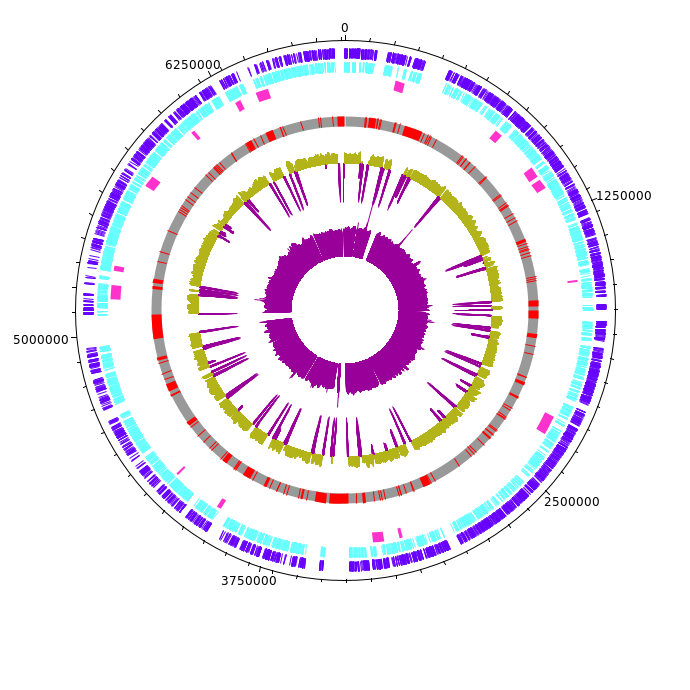
\includegraphics[width=0.8\linewidth]{imagens/genome/002.png} \\
	\centering
    \begin{small}\textbf{Fonte: O Autor (2022)}\end{small}
\end{figure}
\vspace{\floatsep}

\begin{figure}[H]
	\caption{Gráficos representando a montagem do cromossomo da amostra 094}
	\label{fig:genoma94}
	\centering
	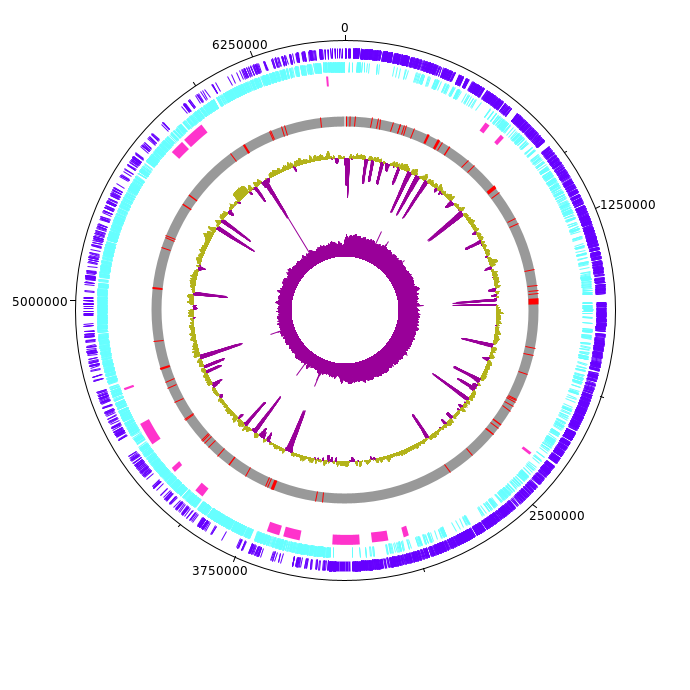
\includegraphics[width=0.8\linewidth]{imagens/genome/004.png} \\
	\centering
    \begin{small}\textbf{Fonte: O Autor (2022)}\end{small}
\end{figure}
\vspace{\floatsep}

As figuras \ref{genoma16}\ref{genoma94} representam as montagens completas dos genomas, sendo
os círculos do mais exterior para interior: Genes na direção \textit{foward} $($ roxo $)$,
Genes na direção \textit{reverse} $($ azul claro $)$, \textit{clusters} gênicos $($ rosa $)$,
qualidade da montagem $($ em cinza a montagem e em vermelho os \textit{gaps} da montagem $)$ e internamente 
um gráfico representando a variação de conteúdo G$+$C $($ amarelo quando maior que 50\% e rosa quando menor$)$ e
mais internamente um gráfico representando o valor de G$+$C. 

Através dessa visualização, podemos observar a sobreposição de alguns clusters gênicos com áreas
de \textit{gaps} na montagem, o que não desqualifica a predição desses clusters mas pode levar
a uma baixa identidades ou ausência de componentes nos clusters como genes acessórios importantes
para a síntese. O aprimoramento da montagem se faz necessário para o depósito desses genomas em 
bancos de dados de montagens. Esse pode ter sido um dos motivos para a baixa identificação dos
cluster na amostra 016.